% !TeX root = ../../Thesis.tex

\chapter{Inflationary stimulated Raman scattering in shock-ignition plasmas}
\label{chp:iSRS}
\bibliographystyle{plainnat}
\nobibliography*

\title{Inflationary stimulated Raman scattering in shock-ignition plasmas}

This chapter is adapted, with the permission of AIP Publishing, from:
\begin{itemize}
  \item \bibentry{Spencer2020}.
\end{itemize}

\section{Motivation and literature review}
\subsection{Homogeneous plasmas}
\subsection{Inhomogeneous plasmas}
test\cite{Vu2001}


\section{Code and initial conditions}\label{sec:code&IC}

\begin{table}[ht]
    \caption{\label{tab:densities}
        Summary of density profiles and $k_{EPW}\lambda_\mathrm{D}$ values in each simulation. $L_n=n_e/(dn_e/dx)$ evaluated at $n_\mathrm{mid}$. For all but the case centred at $0.2n_\mathrm{cr}$, $k_\mathrm{EPW}\lambda_\mathrm{D} > 0.28$ and we are in the strongly kinetic regime. The total range of $k_\mathrm{EPW}\lambda_\mathrm{D}$ probed is 0.21-0.41.
        }
    %\begin{ruledtabular}
    \begin{tabular}{cccc}
    $L_n/\si{\micro \metre}$  & $n_\mathrm{mid}/n_\mathrm{cr}$ & $(n_\mathrm{min},n_\mathrm{max})/n_\mathrm{cr}$ &$(k\lambda_\mathrm{D_{min}},k\lambda_\mathrm{D_{max}})$\\
    \hline
    300& 0.15  & $(0.13,0.18)$ & $(0.28,0.37)$\\
    500 & 0.12 &$(0.11,0.13)$ & $(0.37,0.41)$\\
    500 & 0.15 & $(0.14,0.17)$& $(0.29,0.35)$ \\
    500 & 0.20 & $(0.18,0.22)$& $(0.21,0.27)$\\
    1000 & 0.15 & $(0.14,0.16)$ & $(0.31,0.32)$ \\
    \end{tabular}
    %\end{ruledtabular}
\end{table}

\section{Diagnosing iSRS in inhomogeneous plasmas}\label{sec:signatures}
\subsection{Inflation threshold}

\begin{figure}[ht]
    \centering
    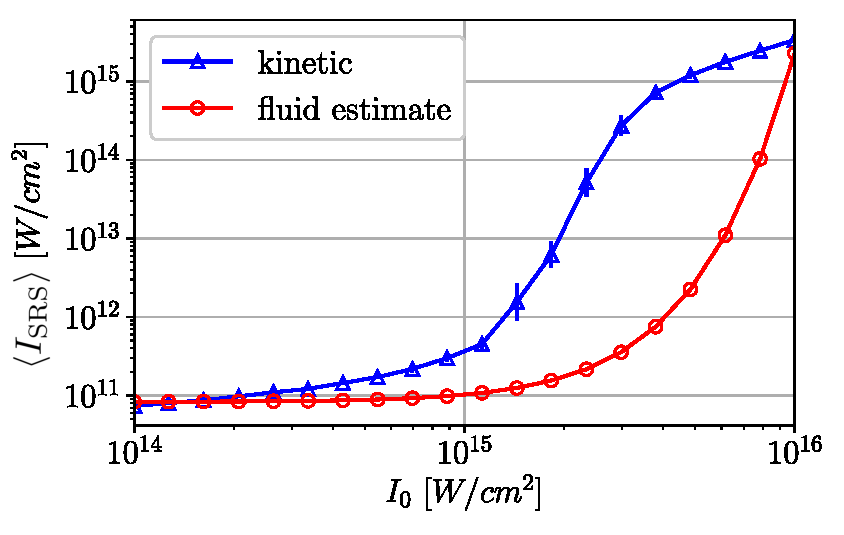
\includegraphics[width=0.8\columnwidth]{Chapters/C4_iSRS/fig2.pdf}
    \caption{
        Blue triangular markers show the intensity of SRS scattered light calculated using the fully-kinetic EPOCH code for parameters: $L_n = 500 \si{\micro\metre} $ and $n_{\mathrm{mid}} = 0.15n_\mathrm{cr}$.
        Red circular markers show the intensity of SRS scattered light calculated, for the same plasma parameters, from the fluid model presented above.
        The initial noise level in the fluid model was calculated from a PIC simulation without the laser driver: $I_\mathrm{noise}=\langle E_yB_z\rangle_{x,t} / \mu_0 = 8\times 10^{10} \si{W/\centi\metre^2}$.}
    \label{fig:kineticVsfluid}
\end{figure}{}

\subsection{Electron trapping}
\subsection{Nonlinear frequency shift}
\subsection{Beam acoustic modes}
%%%%%%%%%%%%%%%%%%%%%%%%%%%%%%%%%%%%%%%%%%%%%%%%%%%%%%%%%%%%%%%%%%%%%%%%%%%%%%%%%%%%%%%%%%
%%                              SEC: THRESHOLD AND HE                                   %%
%%%%%%%%%%%%%%%%%%%%%%%%%%%%%%%%%%%%%%%%%%%%%%%%%%%%%%%%%%%%%%%%%%%%%%%%%%%%%%%%%%%%%%%%%%

\section{Intensity threshold and hot electron scaling}\label{sec:paramScan}

\section{Conclusion}\label{sec:conclusion}

\bibliography{Chapters/C4_iSRS/iSRS}
